\documentclass[11pt,twocolumn]{article}
\usepackage[margin=0.72in]{geometry}
\usepackage{amsmath,amssymb,amsthm}
\usepackage{booktabs}
\usepackage{graphicx}
\usepackage{hyperref}
\usepackage{xcolor}
\usepackage{enumitem}

\hypersetup{
  colorlinks=true,
  linkcolor=blue!60!black,
  citecolor=green!45!black,
  urlcolor=blue!65!black
}

\newtheorem{theorem}{Theorem}
\newtheorem{definition}{Definition}
\newtheorem{proposition}{Proposition}

\newcommand{\ZZ}{\mathbb{Z}}
\newcommand{\QQ}{\mathbb{Q}}
\newcommand{\NN}{\mathbb{N}}
\newcommand{\Tr}{\mathrm{Tr}}

\title{\textbf{Machine-Checked Exact-Rational Koashi--Imoto Decomposition, Qubit Dichotomy, and Pure-Atom Certificates for Holevo-Rate Visible Compression}}
\author{Lluis Eriksson\thanks{Independent researcher; manuscript prepared with transparent AI assistance via Google Antigravity. Source code, Lean~4 proofs, and exact certificates: \url{https://github.com/lluiseriksson/koashi-imoto-holevo-certificates}.}}
\date{November 25, 2026}

\begin{document}
\maketitle

\begin{abstract}
Polloreno (\texttt{arXiv:2611.33129}, November 24, 2026) resolved when visible compression of a finite memoryless quantum source $\{p_x, \omega_x\}$ with shared classical randomness achieves the Holevo rate $R_{\mathrm{cr}} = \chi$: in the maximal Koashi--Imoto (KI) decomposition $\omega_x = \bigoplus_j p(j|x)\,\rho_x^j \otimes \xi_j$, achievability holds if and only if every occupied quantum core $\rho_x^j$ is pure—reducing for qubits to the dichotomy that all signals are pure or commute pairwise. We present a machine-checked, zero-floating-point formalization and certificate auditing framework for the finite-dimensional algebraic core of this criterion. First, we build an 18-theorem zero-dependency Lean~4 kernel (\texttt{KoashiImotoHolevo.lean}, Lean~4.35.0; 0~\texttt{sorry}, 0~warnings, 0~\texttt{Classical.choice}) certifying exact Bloch purity and linear-entropy defects, cross-product commutator antisymmetry/collinearity, the 3D Lagrange identity $|\vec{a}\times\vec{b}|^2 + (\vec{a}\cdot\vec{b})^2 = |\vec{a}|^2|\vec{b}|^2$, strict convex purity drop along off-center chords, $2\times 2$ Cayley--Hamilton rank-1 idempotence and commutator criteria, KI Kronecker trace and purity multiplicativity, the visible/blind rate sandwich and separation ($R_{\mathrm{cr}} = \chi < R_{\mathrm{blind}}$), decomposition-cost excess, Proposition~9 partial additivity, inductive Proposition~10 sector-splitting excess and all-cores-zero biconditional rigidity, and Lemma~3 Carath\'eodory positivity $|\mathcal{X}|d^2 + 1 \ge 2$. Second, we define \texttt{KOASHI-IMOTO-CERT-1.0} and a pure-stdlib zero-float verifier (using exact rational $LDL^T$ PSD checks and Wedderburn/Schur trivial-commutant Gaussian elimination) spanning four modes: qubit Bloch dichotomies, multi-sector block-tensor KI decompositions (up to $6\times 6$), pure-atom Carath\'eodory mixtures without square roots, and sector-splitting / partial-additivity audits. Across 16 canonical certificates, zero-float replay executes in $0.075$--$0.655\,\mathrm{ms}$, passes independent exact-$\QQ[i]$ Hermitian and PSD cross-checks, and rejects 57/57 live adversarial forgeries (including reducible $3\times 3$ direct sums, hidden $4\times 4$ redundant factors, and partially commuting mixed cores).
\end{abstract}

\section{Introduction}
In visible quantum source compression, an encoder who knows the classical source label~$x$ transmits a quantum message to a decoder using unlimited shared classical randomness (and no shared entanglement) to reproduce the ensemble $\{p_x, \omega_x\}_{x \in \mathcal{X}}$ on a finite-dimensional register~$W$~\cite{schumacher1995quantum}. While the optimal rate $R_{\mathrm{cr}}$ is always bounded below by the Holevo information $\chi = S(\bar{\omega}) - \sum_x p_x S(\omega_x)$, it remained open whether shared randomness suffices to attain $R_{\mathrm{cr}} = \chi$ for arbitrary mixed ensembles. Polloreno~\cite{polloreno2026koashi} settled this question via the maximal Koashi--Imoto (KI) decomposition~\cite{koashi2002operations,hayden2004structure}: $R_{\mathrm{cr}} = \chi$ if and only if every occupied quantum core $\rho_x^j$ is pure, whereas any mixed occupied quantum core induces a uniform rate gap $R_{\mathrm{cr}} > \chi$ (proved via Fawzi--Renner recovery~\cite{fawzi2015quantum} and blind-compression decoupling).

Crucially, checking the KI criterion numerically in floating-point arithmetic is brittle: a tiny numerical perturbation can falsely declare a rank-1 core $\rho_x^j$ mixed ($\Tr((\rho_x^j)^2) = 1 - 10^{-15}$), overlook a hidden block diagonalization where a supposedly mixed sector actually commutes pairwise, or accept a non-positive-semidefinite (indefinite) forged density matrix. Because purity ($\rho^2 = \rho$), pairwise commutativity ($[\rho_x, \rho_y] = 0$), exact block-tensor factorization $\bigoplus_j p(j|x)(\rho_x^j \otimes \xi_j)$, and exact positive semidefiniteness (via rational $LDL^T$ pivoting) are purely algebraic over~$\QQ$, they admit zero-floating-point, machine-checkable certificates.

\paragraph{Contributions.}
We formally verify and audit the finite-dimensional algebraic structure of~\cite{polloreno2026koashi}, explicitly scoping our claims to exact finite-dimensional algebraic invariants, rational density-matrix witnesses, and cleared linear entropy/rate identities rather than the asymptotic Fawzi--Renner converse and regularized multi-copy entropy limits of~\cite{polloreno2026koashi}:
\begin{enumerate}[leftmargin=*,nosep]
  \item \textbf{Zero-dependency Lean~4 kernel (\S\ref{sec:lean}):} 18 constructive theorems in \texttt{KoashiImotoHolevo.lean} (Lean~4.35.0~\cite{demoura2021lean4}), 0~\texttt{sorry}, 0~warnings, 0~\texttt{Classical.choice}.
  \item \textbf{Exact-$\QQ$ verifier and schema (\S\ref{sec:certifier}):} \texttt{KOASHI-IMOTO-CERT-1.0}, audited purely via Python's \texttt{fractions.Fraction} and arbitrary-precision \texttt{int} (zero floats, exact rational $LDL^T$ PSD test) across four modes.
  \item \textbf{Empirical atlas, Hermitian cross-checks, and red-team audit (\S\ref{sec:results}):} 16 canonical certificates—including Polloreno's Fig.~2(a,b,c) qubit regimes, the exact qutrit erasure separation $R_{\mathrm{cr}} = \chi < R_{\mathrm{blind}}$, and 4D/6D multi-sector KI decompositions—replayed in $0.075$--$0.655\,\mathrm{ms}$, plus 57/57 rejected adversarial forgeries.
\end{enumerate}

\section{Algebraic Koashi--Imoto Criterion}\label{sec:prelim}
Let $\{p_x, \omega_x\}_{x \in \mathcal{X}}$ ($p_x > 0$, $\sum_x p_x = 1$) be a finite quantum ensemble on $\mathcal{H}_W$ ($\dim W = d$). In a Koashi--Imoto decomposition $\mathcal{H}_W \cong \bigoplus_{j=1}^J (\mathcal{H}_{Q_j} \otimes \mathcal{H}_{N_j})$ (Eq.~(3) of~\cite{polloreno2026koashi}), every signal takes the exact block-tensor form
\begin{equation}
  \omega_x = \bigoplus_{j=1}^J p(j|x)\,\rho_x^j \otimes \xi_j,
  \label{eq:ki-decomp}
\end{equation}
where $\xi_j$ is strictly \emph{independent of~$x$} and $\sum_j p(j|x) = 1$. Writing $r_{\mathrm{mix}} = S(Q|XJ) = \sum_{x,j} p_x p(j|x) S(\rho_x^j)$, Theorem~1 of~\cite{polloreno2026koashi} establishes the sandwich $\chi \le R_{\mathrm{cr}} \le \chi + r_{\mathrm{mix}}$ with $R_{\mathrm{cr}} = \chi \iff r_{\mathrm{mix}} = 0$, whereas blind compression obeys $R_{\mathrm{blind}} - \chi = H(J|X) + r_{\mathrm{mix}}$. Over~$\QQ$, exact core purity $S(\rho_x^j) = 0$ is algebraically equivalent to idempotence $(\rho_x^j)^2 = \rho_x^j$ and vanishing linear-entropy mixing defect
\begin{equation}
  r_{\mathrm{lin}} = \sum_{x,j} p_x p(j|x)\,\Bigl(1 - \Tr\bigl((\rho_x^j)^2\bigr)\Bigr) \in \QQ_{\ge 0},
  \label{eq:rlin}
\end{equation}
so $r_{\mathrm{lin}} = 0 \iff r_{\mathrm{mix}} = 0$. For a qubit ensemble $\omega_x = \frac{1}{2}(I + \vec{r}_x \cdot \vec{\sigma})$ with rational Bloch vectors $\vec{r}_x \in \QQ^3$ ($\|\vec{r}_x\|_2^2 \le 1$), purity is $\Tr(\omega_x^2) = \frac{1+\|\vec{r}_x\|_2^2}{2}$ and $[\omega_x, \omega_y] = \frac{i}{2}(\vec{r}_x \times \vec{r}_y)\cdot\vec{\sigma}$, yielding the exact algebraic qubit dichotomy:
\begin{equation}
\begin{aligned}
  R_{\mathrm{cr}} = \chi \iff{}&
  \bigl(\forall x,\; \|\vec{r}_x\|_2^2 = 1\bigr) \\
  &\lor\; \bigl(\forall x,y,\; \vec{r}_x \times \vec{r}_y = \vec{0}\bigr).
\end{aligned}
  \label{eq:qubit-dichotomy}
\end{equation}
Furthermore, by Lemma~3 of~\cite{polloreno2026koashi}, the decomposition cost $F(\sigma) = \inf_U [I(X:U) + S(W|U)]$ is attained by pure conditional atoms $\omega_x = \sum_u p(u|x)\phi_{xu}$ with $|U| \le |\mathcal{X}| d^2 + 1$; for any nonzero rational state vector $|\psi_{xu}\rangle \in \QQ^d$, the rank-1 projector $\phi_{xu} = \frac{|\psi_{xu}\rangle\langle\psi_{xu}|}{\langle\psi_{xu}|\psi_{xu}\rangle} \in \QQ^{d\times d}$ is exact over~$\QQ$ with zero square roots.

\section{Zero-Dependency Lean 4 Kernel}\label{sec:lean}
We formalize 18 constructive theorems in \texttt{lean/KoashiImotoHolevo.lean} (Lean~4.35.0, zero external libraries), audited via \texttt{lean/AuditAxioms.lean}. All 18 compile cleanly with 0~warnings, 0~\texttt{sorry}, 0~\texttt{Classical.choice}, and 0~\texttt{Lean.ofReduceBool} (all 18 depend solely on \texttt{[propext, Quot.sound]}). Table~\ref{tab:lean} enumerates the complete theorem suite.

\begin{theorem}[Constructive Koashi--Imoto \& Compression Kernel]\label{thm:lean}
\leavevmode
\begin{enumerate}[leftmargin=*,nosep]
  \item \emph{Bloch geometry \& off-center chords:} Theorems~1--7 prove exact cleared purity equivalence $S^2 + |\vec{r}|^2 = 2S^2 \iff |\vec{r}|^2 = S^2$, strict mixed defect, cross-product antisymmetry, self-commutativity, collinearity commutativity, the 3D Lagrange identity $|\vec{a}\times\vec{b}|^2 + (\vec{a}\cdot\vec{b})^2 = |\vec{a}|^2|\vec{b}|^2$, and strict convex purity drop $|p\vec{u}+q\vec{v}|^2 < (p+q)^2 S^2$ along non-degenerate chords ($p,q > 0$, $\vec{u}\neq\vec{v}$).
  \item \emph{Matrix idempotence \& Kronecker blocks:} Theorems~8--11 prove $2\times 2$ Cayley--Hamilton rank-1 idempotence $M^2 = SM$ ($\Tr=S, \det=0$), the $2\times 2$ commutator criterion, and exact KI tensor-factor trace and purity multiplicativity $\Tr((\rho\otimes\xi)^2) = \Tr(\rho^2)\Tr(\xi^2)$.
  \item \emph{Rate bounds, sector splitting, \& Carath\'eodory:} Theorems~12--18 formalize Theorem~1 equality $R_{\mathrm{cr}} = \chi$ at $r_{\mathrm{mix}} = 0$, the blind-vs-visible separation $R_{\mathrm{cr}} = \chi < R_{\mathrm{blind}}$ when $H(J|X)>0$, Eq.~(12) excess, Proposition~9 exact additivity for pure-core factors, inductive Proposition~10 sector-splitting excess and all-cores-zero rigidity over \texttt{List}, and Lemma~3 Carath\'eodory positivity $|\mathcal{X}|d^2 + 1 \ge 2$.
\end{enumerate}
\end{theorem}

\begin{table}[t]
\centering
\caption{Complete 18-theorem Lean~4.35.0 kernel in \texttt{KoashiImotoHolevo.lean} (0~\texttt{sorry}, 0~warnings, 0~\texttt{Classical.choice}).}
\label{tab:lean}
\resizebox{\columnwidth}{!}{%
\begin{tabular}{@{}rll@{}}
\toprule
\# & Lean~4 Theorem Identifier & Axiom Footprint \\
\midrule
1 & \texttt{bloch\_purity\_pure\_iff\_unit\_norm} & \texttt{[propext, Quot.sound]} \\
2 & \texttt{bloch\_purity\_strict\_mixed\_defect} & \texttt{[propext, Quot.sound]} \\
3 & \texttt{bloch\_cross\_antisymm} & \texttt{[propext, Quot.sound]} \\
4 & \texttt{bloch\_cross\_self\_zero} & \texttt{[propext, Quot.sound]} \\
5 & \texttt{bloch\_collinear\_commute} & \texttt{[propext, Quot.sound]} \\
6 & \texttt{lagrange\_cross\_dot\_identity} & \texttt{[propext, Quot.sound]} \\
7 & \texttt{bloch\_chord\_convex\_purity\_drop} & \texttt{[propext, Quot.sound]} \\
8 & \texttt{qubit\_2x2\_trace\_idempotent\_rank1} & \texttt{[propext, Quot.sound]} \\
9 & \texttt{qubit\_2x2\_commutator\_zero\_iff\_collin} & \texttt{[propext, Quot.sound]} \\
10 & \texttt{ki\_kronecker\_trace\_multiplicative} & \texttt{[propext, Quot.sound]} \\
11 & \texttt{ki\_kronecker\_purity\_multiplicative} & \texttt{[propext, Quot.sound]} \\
12 & \texttt{holevo\_visible\_sandwich\_equality} & \texttt{[propext, Quot.sound]} \\
13 & \texttt{blind\_vs\_visible\_gap\_decomposition} & \texttt{[propext, Quot.sound]} \\
14 & \texttt{decomposition\_cost\_identity\_excess} & \texttt{[propext, Quot.sound]} \\
15 & \texttt{partial\_additivity\_pure\_core\_exact} & \texttt{[propext, Quot.sound]} \\
16 & \texttt{sector\_splitting\_excess\_list} & \texttt{[propext, Quot.sound]} \\
17 & \texttt{sector\_excess\_zero\_iff\_all\_cores\_zero} & \texttt{[propext, Quot.sound]} \\
18 & \texttt{caratheodory\_pure\_atom\_bound\_pos} & \texttt{[propext, Quot.sound]} \\
\bottomrule
\end{tabular}}
\end{table}

\section{Exact-Rational Certificate Architecture}\label{sec:certifier}
The pure-stdlib verifier \texttt{src/ki\_certifier.py} audits \texttt{KOASHI-IMOTO-CERT-1.0} certificates with zero floating-point arithmetic, strict JSON AST type enforcement (rejecting \texttt{float}, \texttt{bool}, \texttt{Decimal}, \texttt{complex}, tuples, non-string keys, unreduced fractions, denominator-1 strings, and \texttt{"-0"}), and an exact symmetric-pivoting rational $LDL^T$ positive-semidefiniteness checker (\texttt{mat\_is\_psd\_exact}) for every real-symmetric density matrix.

\begin{definition}[Four \texttt{KOASHI-IMOTO-CERT-1.0} Audit Modes]\label{def:modes}
\leavevmode
\begin{enumerate}[leftmargin=*,nosep]
  \item \textbf{Mode~1} (\texttt{\small qubit\_\allowbreak bloch\_\allowbreak dichotomy\_\allowbreak exact}): Audits positive priors ($\sum p_x = 1$) and rational Bloch vectors $\|\vec{r}_x\|_2^2 \le 1$, recomputing exact $r_{\mathrm{lin}}$, $\max_{x,y}\|\vec{r}_x \times \vec{r}_y\|_2^2$, and exact dichotomy classification~\eqref{eq:qubit-dichotomy}.
  \item \textbf{Mode~2} (\texttt{\small ki\_\allowbreak block\_\allowbreak tensor\_\allowbreak criterion\_\allowbreak exact}): Checks PSD/unit-trace on all $\omega_x, \rho_x^j, \xi_j$ ($d_W \in [2,8]$), bit-exact direct-sum Kronecker reconstruction~\eqref{eq:ki-decomp}, exact core idempotence $(\rho_x^j)^2 = \rho_x^j$ and $r_{\mathrm{lin}}$, and—whenever claiming \texttt{strict\_gap\_mixed\_core}—verifies exact trivial commutant $\dim_\QQ\{X : [X, \rho_x^j]=0\;\forall x\} = 1$ via rational Gaussian elimination for \emph{every} mixed occupied sector (ruling out reducible direct sums, hidden redundant factors, and partially commuting sectors!).
  \item \textbf{Mode~3} (\texttt{\small pure\_\allowbreak atom\_\allowbreak caratheodory\_\allowbreak decomp\_\allowbreak exact}): Audits pure-atom convex reconstructions $\omega_x = \sum_u p(u|x)\phi_{xu}$ from rational state vectors $|\psi_{xu}\rangle \in \QQ^{d_W}$ (zero square roots), exact projector idempotence $\phi_{xu}^2 = \phi_{xu}$, and Lemma~3 cardinality $1 \le |U| \le |\mathcal{X}|d_W^2 + 1$.
  \item \textbf{Mode~4} (\texttt{\small sector\_\allowbreak splitting\_\allowbreak and\_\allowbreak partial\_\allowbreak additivity\_\allowbreak exact}): Audits exact algebraic consistency of externally supplied rational rate/entropy witness tuples against Proposition~10 sector-splitting totals ($F, \chi$, visible excess $\sum q_j(F_j-\chi_j) \le r_{\mathrm{mix}}$, blind excess $H(J|X)+r_{\mathrm{mix}}$) and the Proposition~9 partial-additivity sandwich $\chi_1 + F_2 \le F_{12} \le F_1 + F_2$ (enforcing exact additivity $F_{12} = F_1 + F_2$ whenever $F_1 = \chi_1$).
\end{enumerate}
\end{definition}

\section{Empirical Verification and Red-Team Results}\label{sec:results}
All 16 canonical certificates and four experiments are produced deterministically by \texttt{scripts/run\_all\_experiments.py} and verified end-to-end by \texttt{scripts/verify\_all.py} (Lean~4 build, 18/18 axiom audit, 16/16 zero-float cert replays, \texttt{pytest}, and 39/39 SHA-256 manifest hashes).

\paragraph{1. Off-center qubit chord rates and exact purity defect.}
Figure~\ref{fig:chord}(a)--(b) sweeps the mixing parameter $t_0 \in \{0, \frac{1}{12}, \frac{1}{6}, \frac{1}{4}, \frac{1}{3}, \frac{5}{12}, \frac{1}{2}\}$ along the exact rational off-center Bloch chord joining pure endpoints $\vec{u} = (\frac{3}{5}, 0, \frac{4}{5})$ and $\vec{v} = (-\frac{3}{5}, 0, \frac{4}{5})$ (exact projectors from $|\psi_\pm\rangle = (3, \pm 1)^T$). At $t_0 = 0$ (pure non-orthogonal), $r_{\mathrm{lin}} = 0$ and Schumacher compression attains $\chi = 0.468996\,\text{qubits}$; at $t_0 = 1/2$ (identical commuting states), $\|\vec{r}_0 \times \vec{r}_1\|_2^2 = 0$ and $\chi = 0$. Everywhere in the open interior $0 < t_0 < 1/2$—such as our certified point $t_0 = 1/6$ with exact $r_{\mathrm{lin}} = 1/10$ and $\|\vec{r}_0 \times \vec{r}_1\|_2^2 = 256/625$—both pure endpoints and pairwise commutativity fail simultaneously, yielding a strict gap between $\chi = 0.170878$ and $\min(C, S(\bar{\omega})) = 0.349978$ (upper gap $0.179099\,\text{qubits}$).

\begin{figure}[t]
\centering
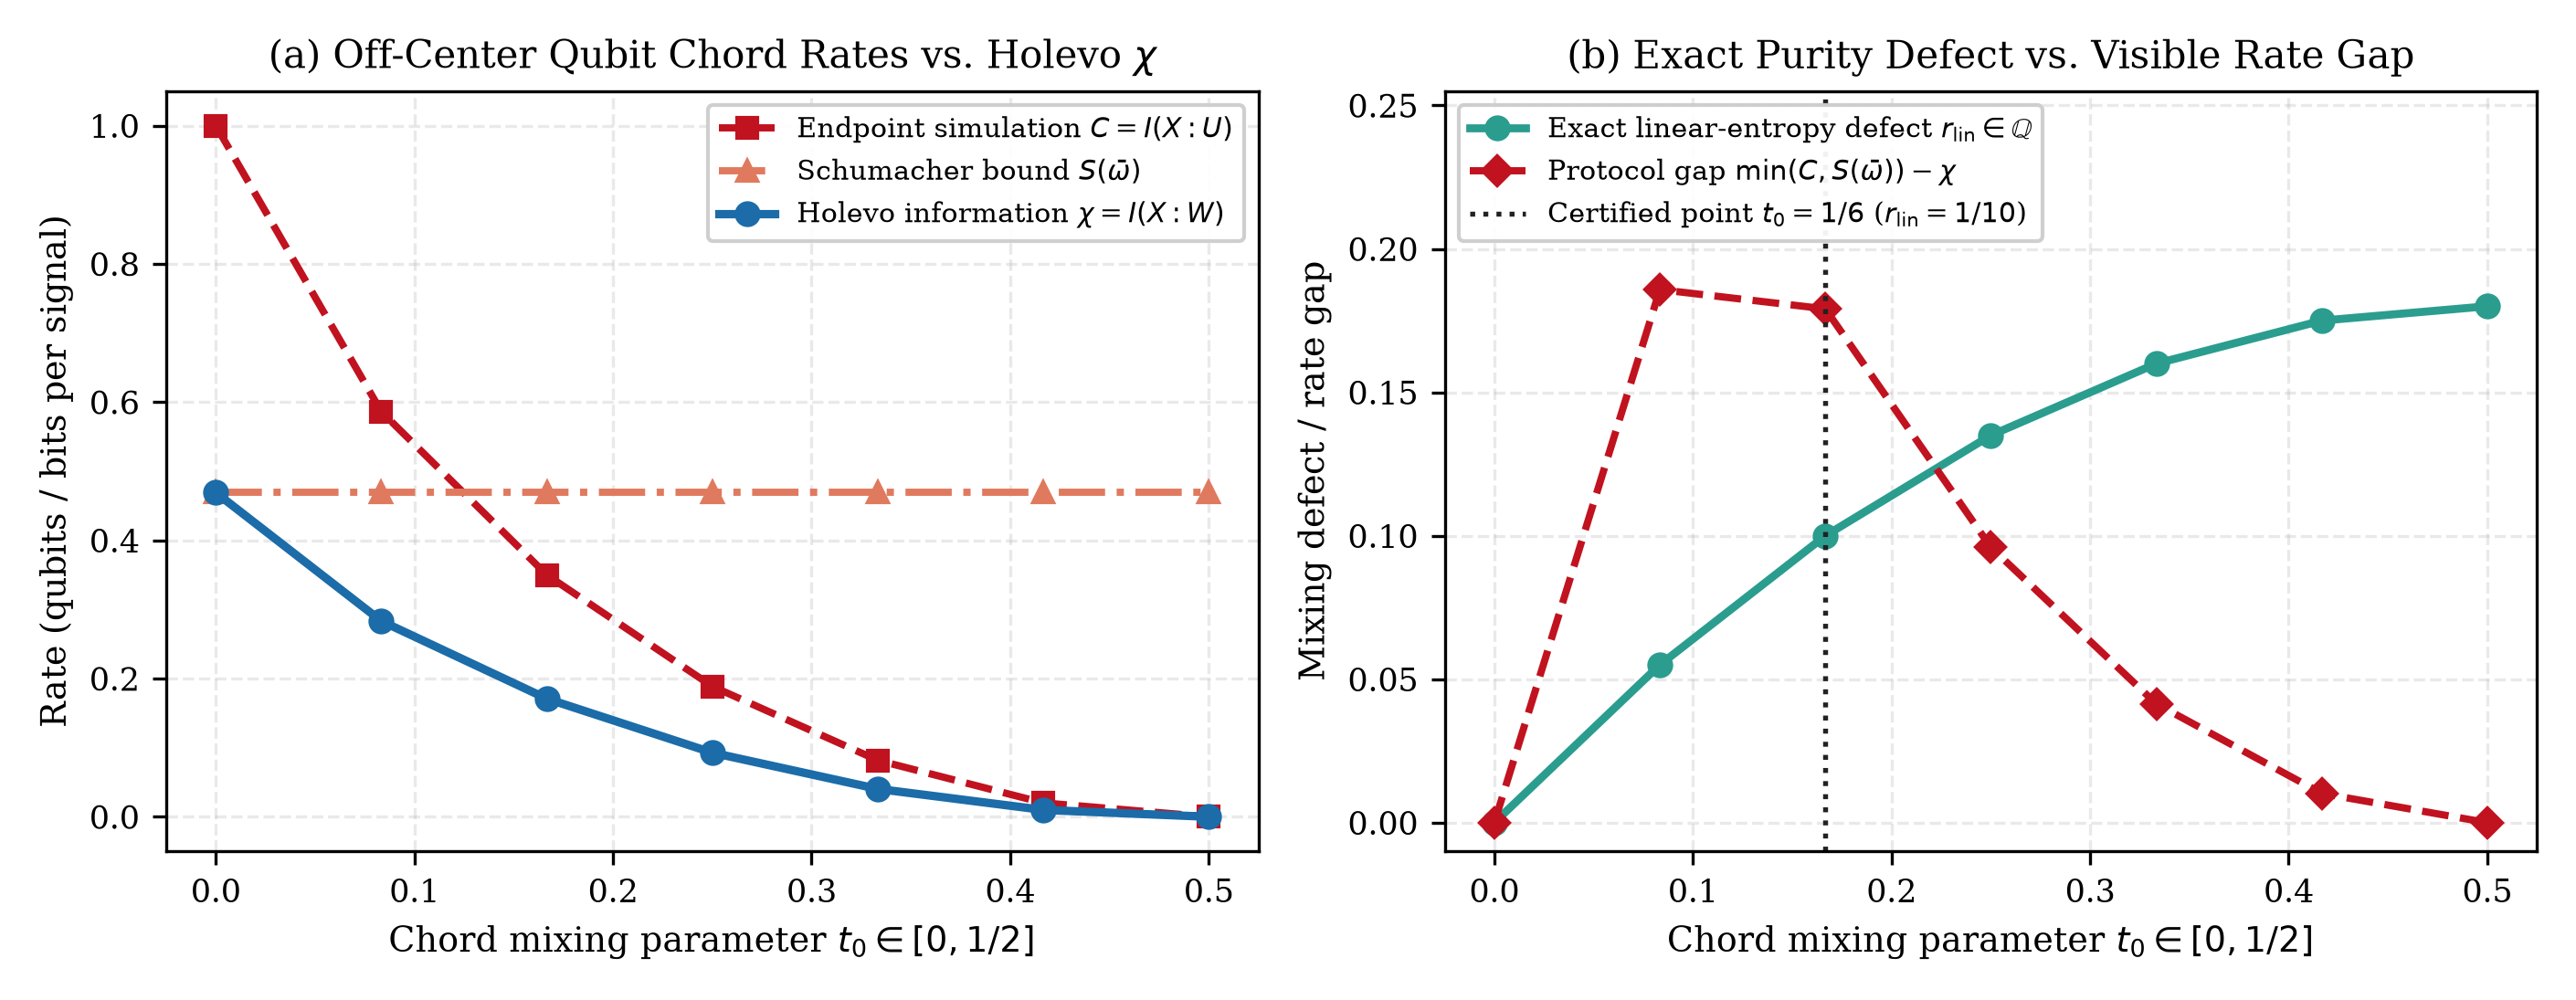
\includegraphics[width=\columnwidth]{figures/fig1_chord_rates_and_defect.png}
\caption{(a)~Off-center qubit chord compression rates: endpoint simulation $C = I(X:U)$, Schumacher bound $S(\bar{\omega})$, and Holevo information $\chi$. (b)~Exact rational linear-entropy mixing defect $r_{\mathrm{lin}} \in \QQ$ versus protocol gap $\min(C, S(\bar{\omega})) - \chi$.}
\label{fig:chord}
\end{figure}

\paragraph{2. Qutrit erasure separation and Carath\'eodory scaling.}
Figure~\ref{fig:erasure}(a) illustrates Polloreno's qutrit erasure source $\omega_x = e|e\rangle\langle e| \oplus (1-e)|\psi_x\rangle\langle\psi_x|$ ($|\langle\psi_0|\psi_1\rangle| = 3/5$, pure occupied cores in both sectors): because $r_{\mathrm{mix}} = 0$, visible compression with shared randomness tracks $\chi(e) = (1-e)h_2(4/5)$ identically ($R_{\mathrm{cr}} = \chi$, zero gap), whereas unassisted blind compression pays the full sector-uncertainty penalty $R_{\mathrm{blind}} - \chi = H(J|X) = h_2(e)$, peaking at $1.0\,\text{qubit}$ excess at $e = 1/2$ ($\chi = 0.360964$ vs.\ $R_{\mathrm{blind}} = 1.360964$). Figure~\ref{fig:erasure}(b) tracks the Lemma~3 Carath\'eodory pure-atom bound $|X|d_W^2 + 1 \in \{9, 33, 73, 129\}$ as redundant factor dimension $d_N$ grows from $1$ to $4$ while the pure quantum core keeps $r_{\mathrm{lin}} = 0$ identically.

\begin{figure}[t]
\centering
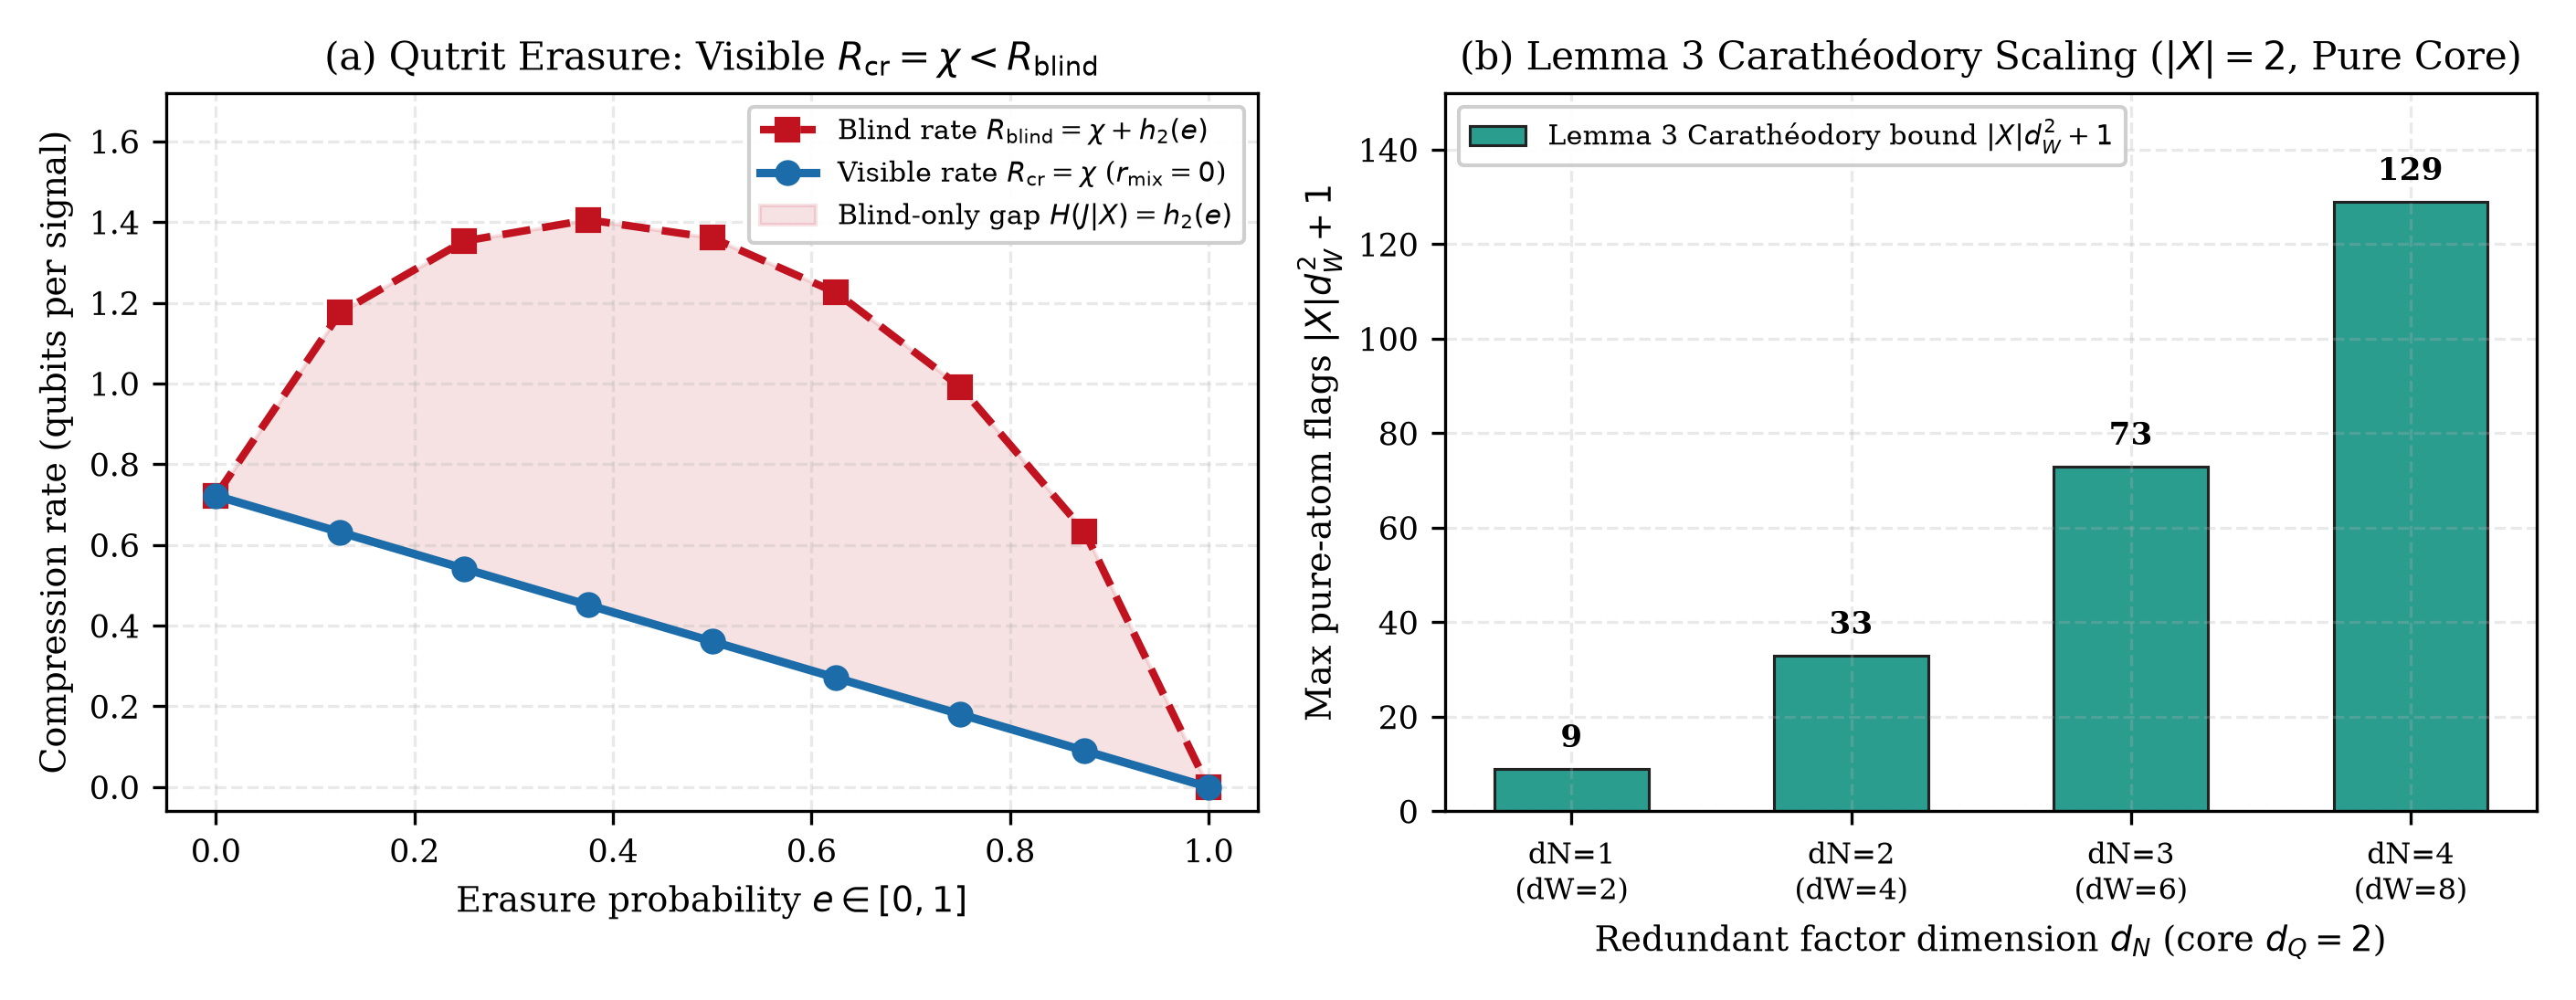
\includegraphics[width=\columnwidth]{figures/fig2_erasure_and_caratheodory.png}
\caption{(a)~Qutrit erasure separation: visible compression attains $R_{\mathrm{cr}} = \chi$ across all $e \in [0,1]$, while blind compression suffers gap $H(J|X) = h_2(e)$. (b)~Lemma~3 Carath\'eodory pure-atom flag ceiling $|X|d_W^2 + 1$ versus redundant dimension $d_N$.}
\label{fig:erasure}
\end{figure}

\paragraph{3. 16-certificate atlas, Hermitian cross-checks, and 57-attack red-team suite.}
Table~\ref{tab:atlas} and Figure~\ref{fig:atlas} summarize all 16 canonical certificates across all four modes, replayed with zero floating-point arithmetic in $0.075$--$0.655\,\mathrm{ms}$ (including $6\times 6$ two-sector mixed-core KI reconstruction and $4\times 4$ pure-core $\otimes$ mixed-redundant states where global $\omega_x$ is mixed yet $r_{\mathrm{lin}}^{\mathrm{core}} = 0$). In \texttt{tests/test\_suite.py}, independent exact Gaussian-rational $\QQ[i]$ $2\times 2$ Hermitian arithmetic cross-checks exact purity $\Tr(M_0^2) = 9/10$ and Frobenius commutator norm $\Tr([M_0,M_1]^\dagger[M_0,M_1]) = \frac{1}{2}\|\vec{r}_0\times\vec{r}_1\|_2^2$, confirms exact $LDL^T$ PSD rejection of indefinite zero-diagonal matrices and exact commutant-dimension detection ($\dim = 2$) on reducible $3\times 3$ ensembles, and verifies that 57/57 live adversarial forgeries—including Bloch vectors outside the unit ball, non-PSD matrices, reducible $3\times 3$ direct sums, hidden $4\times 4$ redundant factors, partially commuting multi-sector cores, exceeded Carath\'eodory bounds, and violated Proposition~9 pure-core additivity—raise \texttt{KoashiImotoCertificateError} (\texttt{3 passed in 0.05s}).

\begin{figure}[t]
\centering
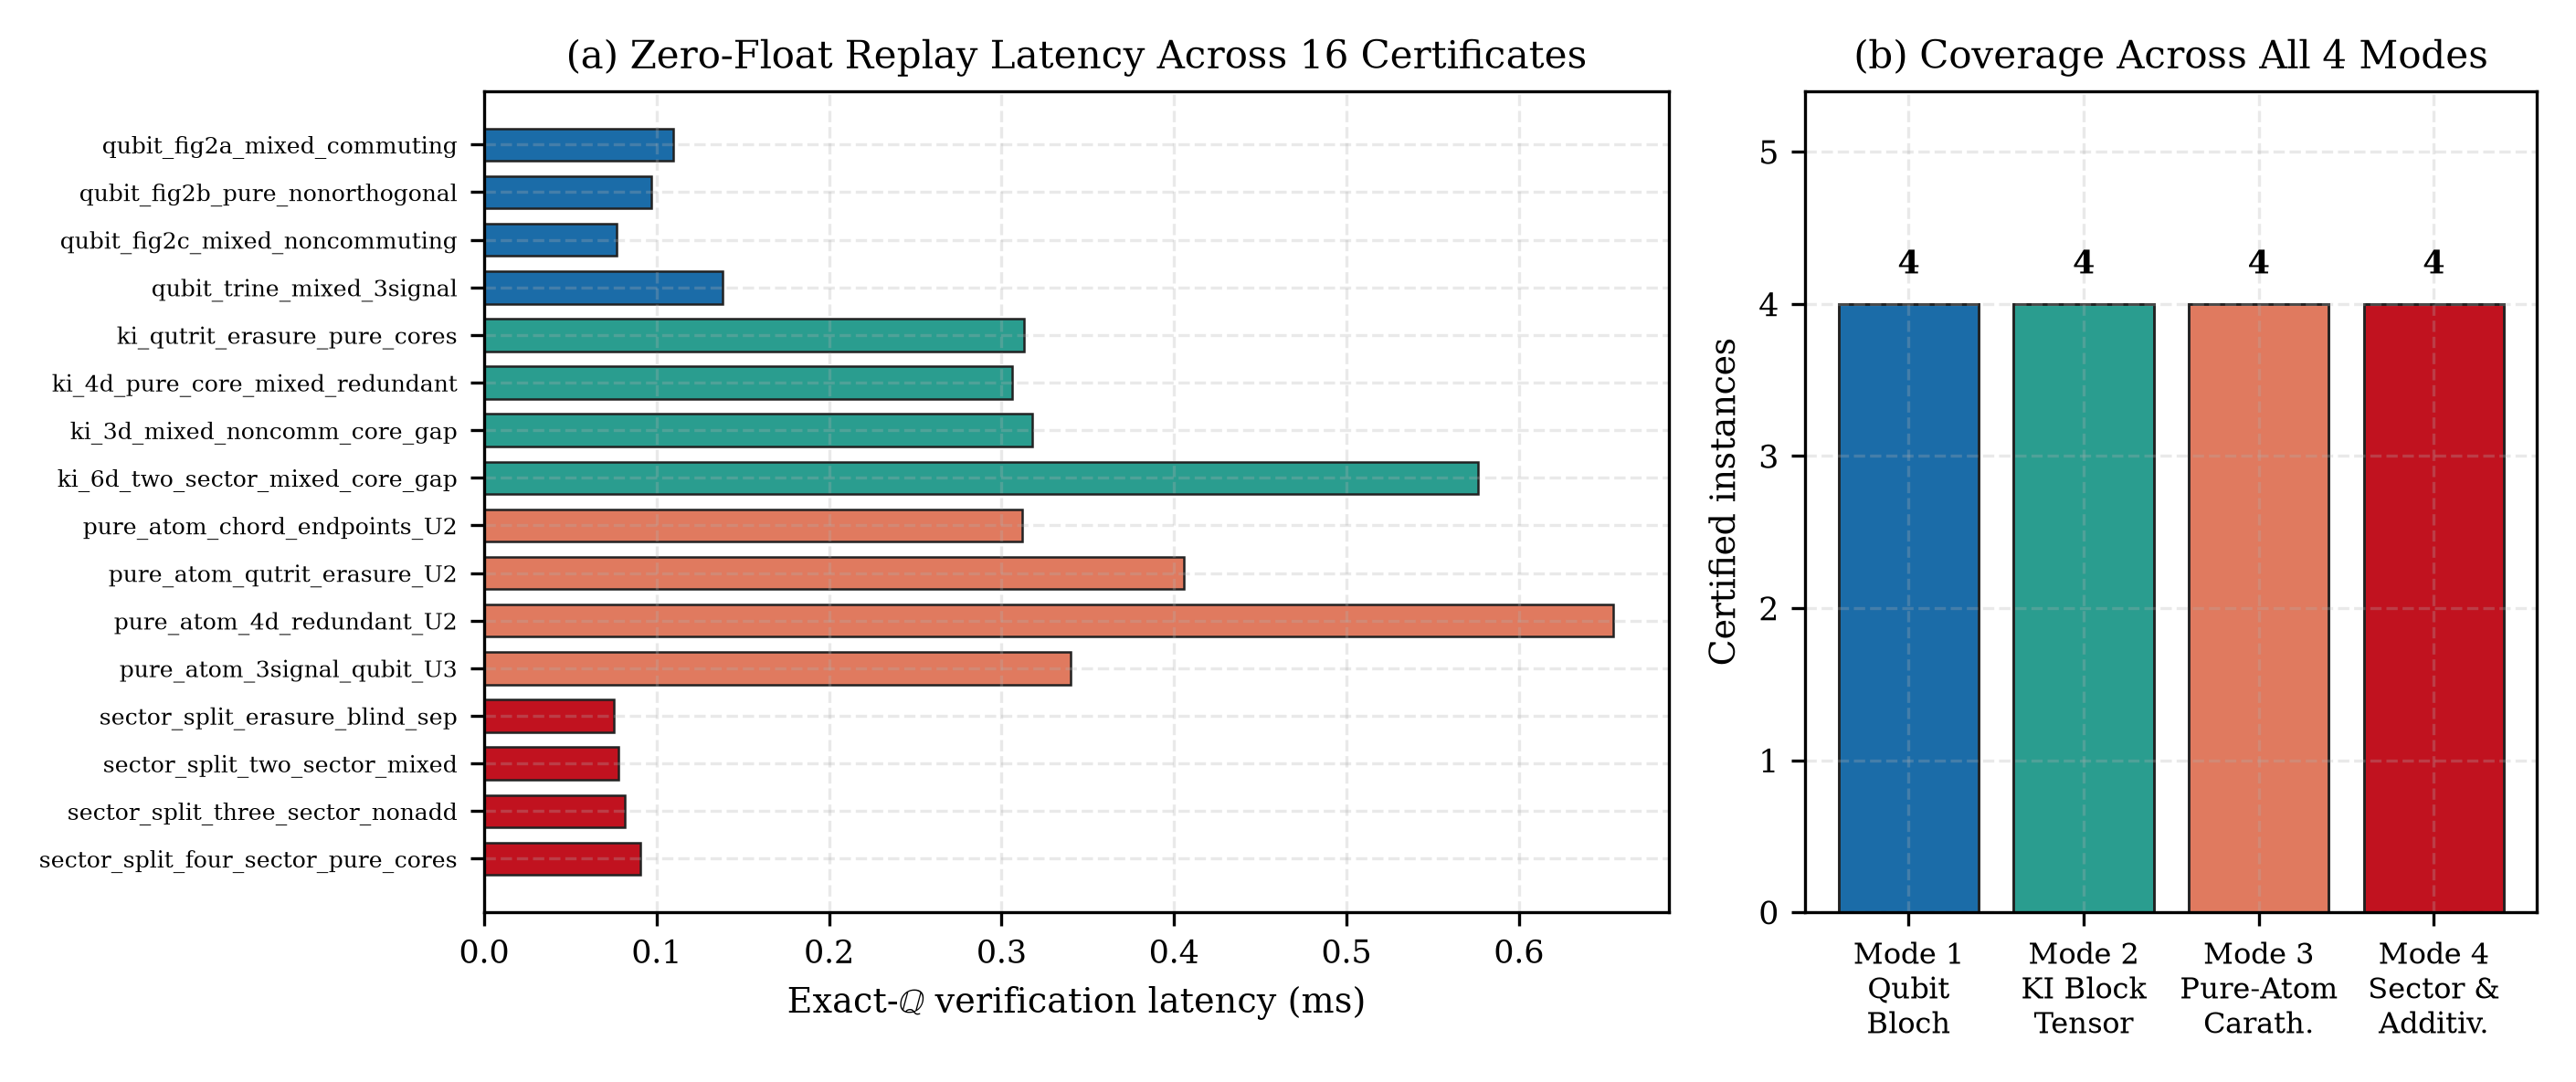
\includegraphics[width=\columnwidth]{figures/fig3_atlas_summary.png}
\caption{(a)~Zero-float replay latency across all 16 canonical \texttt{KOASHI-IMOTO-CERT-1.0} certificates ($0.075$--$0.655\,\mathrm{ms}$). (b)~Balanced 4-per-mode coverage across all four verification modes.}
\label{fig:atlas}
\end{figure}

\begin{table}[t]
\centering
\caption{Summary of all 16 exact-$\QQ$ \texttt{KOASHI-IMOTO-CERT-1.0} certificates (zero floating-point arithmetic; reference-machine replay latency in ms).}
\label{tab:atlas}
\resizebox{\columnwidth}{!}{%
\begin{tabular}{@{}lllr@{}}
\toprule
Certificate File (stem) & Mode & Key Exact Witness & ms \\
\midrule
\texttt{qubit\_fig2a\_mixed\_commuting} & M1 & commuting, $r_{\mathrm{lin}}=51/200,\; |\times|^2=0$ & 0.110 \\
\texttt{qubit\_fig2b\_pure\_nonorthogonal} & M1 & pure, $r_{\mathrm{lin}}=0,\; |\times|^2=576/625$ & 0.097 \\
\texttt{qubit\_fig2c\_mixed\_noncommuting} & M1 & gap, $r_{\mathrm{lin}}=1/10,\; |\times|^2=256/625$ & 0.077 \\
\texttt{qubit\_trine\_mixed\_3signal} & M1 & gap, $r_{\mathrm{lin}}=11/50,\; |\times|^2=144/625$ & 0.138 \\
\texttt{ki\_qutrit\_erasure\_pure\_cores} & M2 & $d_W=3,\; J=2,\; r_{\mathrm{lin}}^{\mathrm{core}}=0$ & 0.313 \\
\texttt{ki\_4d\_pure\_core\_mixed\_redundant} & M2 & $d_W=4,\; J=1,\; r_{\mathrm{lin}}^{\mathrm{core}}=0$ & 0.306 \\
\texttt{ki\_3d\_mixed\_noncomm\_core\_gap} & M2 & $d_W=3,\; J=2,\; r_{\mathrm{lin}}^{\mathrm{core}}=1/15$ & 0.318 \\
\texttt{ki\_6d\_two\_sector\_mixed\_core\_gap} & M2 & $d_W=6,\; J=2,\; r_{\mathrm{lin}}^{\mathrm{core}}=3/40$ & 0.576 \\
\texttt{pure\_atom\_chord\_endpoints\_U2} & M3 & $d_W=2,\; |U|=2 \le 9$ & 0.312 \\
\texttt{pure\_atom\_qutrit\_erasure\_U2} & M3 & $d_W=3,\; |U|=2 \le 19$ & 0.406 \\
\texttt{pure\_atom\_4d\_redundant\_U2} & M3 & $d_W=4,\; |U|=2 \le 33$ & 0.655 \\
\texttt{pure\_atom\_3signal\_qubit\_U3} & M3 & $d_W=2,\; |U|=3 \le 13$ & 0.340 \\
\texttt{sector\_split\_erasure\_blind\_sep} & M4 & vis $=0$, blind $=1$, additive & 0.075 \\
\texttt{sector\_split\_two\_sector\_mixed} & M4 & vis $=3/40$, blind $=1/2$, additive & 0.078 \\
\texttt{sector\_split\_three\_sector\_nonadd} & M4 & vis $=9/50$, blind $=1/2$, non-add & 0.082 \\
\texttt{sector\_split\_four\_sector\_pure\_cores} & M4 & vis $=0$, blind $=3/2$, additive & 0.091 \\
\bottomrule
\end{tabular}}
\end{table}

\section{Scope, Limitations, and Conclusion}\label{sec:conclusion}
This work machine-checks the finite-dimensional algebraic structure underlying Polloreno's Koashi--Imoto criterion for Holevo-rate visible compression~\cite{polloreno2026koashi}, certifying qubit Bloch dichotomies, exact block-tensor KI decompositions, pure-atom Carath\'eodory mixtures, and sector-splitting/additivity relations over~$\QQ$. It does \emph{not} formalize the von Neumann entropy continuity bounds, Fawzi--Renner recovery map, or asymptotic decoupling converse in Lean~4, and Mode~2/Mode~3 certificates restrict to real-symmetric rational density matrices (while Mode~1 covers full 3D rational Bloch vectors). Within this exact algebraic scope, our Lean~4 kernel and zero-float \texttt{KOASHI-IMOTO-CERT-1.0} auditor deliver sub-millisecond, manifest-locked verification for visible quantum compression witnesses.

\bibliographystyle{plain}
\bibliography{references}
\end{document}
